\chapter{Resultados}
A continuación se muestran los resultados obtenidos de la simulación presentada en la sección anterior. En general, por cada archivo de salida de datos (cada 15 minutos en este caso), se obtienen valores de velocidad, presión, temperatura, humedad, TKE, flujo superficiales, entre otras cantidades que utiliza el modelo en cada punto de la malla desplazada. Sin embargo acá no se presentan tantos datos. La muestra de datos se restringe entonces a mostrar de manera cuantitativa el comportamiento dinámico del flujo en la capa límite del dominio mas fino.
\section{Campos Medios de Velocidad}
\section{Perfiles de Velocidad}
\section{Series de Tiempo}
\section{Espectro de Energía}
\newcommand{\spectrafig}[1]{
\begin{figure}[H]
	\centering
	\includegraphics[width=0.9\linewidth,page=#1]{Imagenes/spectra}
	\vspace{-5mm} 
	%\caption{}
	%\label{}
\end{figure}
}
\spectrafig{1}
\spectrafig{2}
\spectrafig{3}
\spectrafig{4}
\spectrafig{5}
\spectrafig{6}
\spectrafig{7}
\spectrafig{8}
\spectrafig{9}
\spectrafig{10}
\spectrafig{11}
\spectrafig{12}
\spectrafig{13}
\spectrafig{14}
\spectrafig{15}
\chapter{Análisis y Conclusiones}